\documentclass{article}
\usepackage{hyperref}
\usepackage{graphicx}
\graphicspath{ {images/} }
\hypersetup{
    colorlinks=true,
    linkcolor=blue,
    filecolor=magenta,      
    urlcolor=blue,
}
\urlstyle{same}
\linespread{1.25}
\begin{document}
\begin{center}
{\Huge Live Audio Commentary\\[5cm]}

{\Large Sam Mai

BSc Computer Science

Submission Date: \today

Supervisor: Harry Strange}
\end{center}
\newpage
Contents
\begin{itemize}
    	\item [1] Introduction
	\begin{itemize}
		\item [1.1] The Problem
		\item [1.2] Why I chose this project?
		\item [1.3] The Challenges
		\item [1.4] Aims and Goals
		\begin{itemize}
			\item [1.4.1] Aims
			\item [1.4.2] Goals
		\end{itemize}
		\item [1.5] How the project was conducted
		\item [1.6] Structure of this report
	\end{itemize}
    	\item [2] Background Information
	\begin{itemize}
		\item [2.1] Sources of Information
		\begin{itemize}
			\item [2.1.1] Android Developers
			\item [2.1.2] Android Login and Registration with PHP, MySQL and SQLite
			\item [2.1.3] Retrofit - Getting Started and Creating an Android Client
			\item [2.1.4] How to Create an Android Chat App Using Firebase
			\item [2.1.5] Android Sliding Menu using Navigation Drawer
			\item [2.1.6] Stack Overflow
		\end{itemize}
		\item [2.2] Similar Products
		\item [2.3] Supporting Tools and Libraries
		\begin{itemize}
			\item [2.3.1] Retrofit API
			\item [2.3.2] Wowza GoCoder SDK
			\item [2.3.3] JW Player SDK
			\item [2.3.4] Firebase API
		\end{itemize}
	\end{itemize}
    	\item [3] Requirements and Analysis
	\begin{itemize}
		\item [3.1] Requirements
		\item [3.2] Use Cases
		\begin{itemize}
			\item [3.2.1] Use Case Diagram
			\item [3.2.2] Use Case Titles
		\end{itemize}
		\item [3.3] Entity-Relationship (ER) Diagram
	\end{itemize}
	\item [4] Design and Implementation
	\begin{itemize}
		\item [4.1] System Architecture
		\item [4.2] Data Flow Diagram
		\item [4.3] Application Components
		\begin{itemize}
			\item [4.3.1] Broadcasting to Streaming Server
			\begin{itemize}
				\item [4.3.1.1] Audio Sampling Rate
			\end{itemize}
			\item [4.3.2] Database
			\begin{itemize}
				\item [4.3.2.1] Structure
				\item [4.3.2.2] Implementation
			\end{itemize}
			\item [4.3.3] Location Service
			\item [4.3.4] Connecting to Server Side
		\end{itemize}
		\item [4.4] Server Components
		\begin{itemize}
			\item [4.4.1] Server Database
			\begin{itemize}
				\item [4.4.1.1] Structure
				\item [4.4.1.2] Implementation
			\end{itemize}
		\end{itemize}
	\end{itemize}
	\item [5] Testing
	\begin{itemize}
		\item [5.1] Testing Strategy
		\begin{itemize}
			\item [5.1.1] Unit Testing
			\item [5.1.2] Functional Testing
			\item [5.1.3] Acceptance Testing
		\end{itemize}
		\item [5.2] Summary
	\end{itemize}
	\item [6] Conclusion and Evaluation
	\begin{itemize}
		\item [6.1] Summary of Achievements
		\item [6.2] Evaluation
		\item [6.3] Future Developments
		\item [6.4] Conclusions
	\end{itemize}
	\item [7] Appendices
	\begin{itemize}
		\item [7.1] Requirements Document
		\item [7.2] Ues Cases
		\item [7.3] Application User Manual / Class Listings
		\item [7.4] System Overview
		\item [7.5] References
	\end{itemize}
\end{itemize}
\newpage
\begin{flushleft}
{\huge Chapter 1: Introduction}\\[0.5cm]
{\Large 1.1 The Problem}\\
Football is one of the most anticipated sports around the world and due to its popularity, football fans often find it hard to follow every single match in a season for numerous reasons be it travel distance, ticket price, accessibility to content etc. To overcome the problem, people may decide to sit around pubs where they can watch the match or if people have access to a computer, streaming from different sources can also be considered a temporary solution. Of course, these solutions are not perfect and it kills the fun of watching football because of the lack of interactions between the fans which is what football is about.\\
In summary, it's hard for football fans to enjoy the sport they love so much without compromising different important aspects of their lives.\\
{\Large 1.2 Why I chose this project?}\\
I chose this project because this is the problem that my family members also experience a lot and it can be quite frustrating to certain people hence needs to be resolved.\\
Apart from that, I also feel that this is the perfect opportunity to learn and improve my technical capability by tackling new areas which I have little to no experience in.\\
Furthermore, not only helping those that don't have frequent access to football matches but the application will also draw people with access to the game by allowing them to socialise with other while giving their thoughts and insights of the game under the form of streaming.\\
{\Large 1.3 The Challenges}\\
1) The first challenge is to ensure that the commentary reflects what's actually happening during the match. It's obviously not possible to ensure every single detail is correct and stream monitoring would cost a lot, not mentioning it's also not technically feasible. However, there are partial solutions to ensure the commentary reports what's actually happening during the match by ensuring the commentator is actually present in the stadium at the time.\\
2) Another challenge is the quality of the audio stream, this is compromised by a lot of factors mainly due to different sample rate supported by different devices and the amount of data used for different sample rate (Keeping in mind this is outside where Wi-Fi is not available so the amount of data is limited).\\
{\Large 1.4 Aims and Goals}\\
{\large 1.4.1 Aims}\\
To develop an Android application where football fans can interact with each other. The application will allow users to listen to live audio commentaries hosted by other users, more specifically commentators. Users can share their own thoughts and insights by registering to become a commentator and record their own commentaries while others can also give feedback by submitting comments at the same time.\\
{\large 1.4.2 Goals}\\\
\begin{itemize}
	\item To allow users to follow football games from others’ points of view through live commentaries.
	\item To allow users to share their thoughts and insights about football games through live commentaries.
	\item To allow users to express their views on quality of commentaries from different commentators.
	\item To offer practices to users who are interested in doing audio commentaries.
	\item To allow users to interact with each other in a friendly manner
\end{itemize}
{\Large 1.5 How the project was conducted}\\
An interative approach was followed thorughout the duration of the project. Firstly, the initial version is a working product with only basic functionalities, then further improvements and extra functionalities are added in every increment leading all the way up until the end of the project.\\
The project plan highlights the durations for each functionality and different phases of the project. The project plan was later revised in the interim report to make sure everything is going well according to the initial plan and whether there were changes to be made.\\
Meetings with supervisor is also scheduled weekly to report back progress made during the past week, this is also the opportunity to raise any concerns and also ask for feedback for the progression and quality of work. Tasks to be done for the upcoming week will also be discussed here as a collaborative effort.\\
{\Large 1.6 Structure of this report}\\
Following this Introduction chapter, the report will then be followed with 5 more chapters. Chapter 2 will be covering background information and related work. This outlines all the main sources of information of related technologies used during the project. Chapter 3 is Requirements and Analysis which discusses all the work done prior to the implementation period of the project. Chapter 4 covers  all the design and implementation strategies, often there will be more than one of way of implementing a certain functionality, this chapter will also be debating related strategies and weigh up their pros and cons. Next up, chapter 5 will go over all the testing strategies performed and the results. Finally, the final chapter 6 will be the conclusion and evaluation that highlights all notable achievements, also what worked well and what didn't and future improvements to be made to the final product.\\
{\huge Chapter 2: Background Information}\\[0.5cm]
{\Large 2.1 Sources of Information}\\
Building a streaming Android application often involves a lot of different technologies and large proportion of time during project was spent on researching about these technologies and their alternatives to find the most suitale product that will fit with the purpose of the project. Details about these technologies will be discussed in the upcoming sections.\\
{\large 2.1.1 Android Developers}\\
Application development in Android is quite complex in comparison to iOS due to the vast variety of products in the market so different screen sizes, solutions, Android versions etc. should be managed well. Furthermore, due to its popularity Android is growing incredibly fast, big codename versions are rolled out every year while small upgrades come out every few months. Android developers\textsuperscript{1} offers a comprehensive guide for Android developers of all levels with frequent updates to help users stay up to date with newer versions of Android. The site also demonstrates best practices for some of the most important aspects such as performance, user input or battery etc.  \\
{\large 2.1.2 Android Login and Registration with PHP, MySQL and SQLite\textsuperscript{2}}\\
This guide shows an example of how to add a very basic user authentication functionality with PHP, MySQL and SQLite. The guide is quite user friendly espeically to developers that are new to PHP and MySQL, explanations are provided from beginning to the end including installations of used software. This also demonstrates an overview of how to manage session data using SharedPreferences, in this case it provides a way to manage user log in session. Furthermore, the guide also introduces the use of SQLite database within Android to store personal information such as name, email, etc. This allows the application to access certain information even when device is not connected to the Internet and also reduces delays when requesting for unimportant information, in this case that would be name, email, commentator status etc. In addition, the author also presents very good practices when calling MySQL statements from PHP, more specifically protection against SQL injection. Talking about security, the guide also provides good practice in dealing with user login credentials which is to store the encrypted password and the salt used to encrypt that password instead of the actual password. This way it is harder to actually crack these passwords without knowledge of salting and encryption algorithms used.
{\large 2.1.3 Retrofit — Getting Started and Creating an Android Client\textsuperscript{3}}\\
This tutorial aims at providing users a walkthrough on how to use Retrofit - Type-safe HTTP client for Android and Java, from configuring the library to more advanced functionalities such as Pagination etc. This tutorial provides comprehensive steps on making synchronous and asynchronous requests with logging so users can actually see what's being returned from a request call. This tutorial is very straightforward with little to no jargons particularly suitable for new Android developers. Moreover, Android Studio users can conveniently use the library after adding a few dependencies on build gradle. 
{\large 2.1.4 How to Create an Android Chat App Using Firebase\textsuperscript{4}}\\
This tutorial shows developers how to create a messaging app using Firebase Cloud Messaging (FCM). As Google Cloud Messaging (GCM) is slowly switching over to Firebase, this tutorial is the perfect example of how Firebase is much more versatile than GCM. The tutorial makes the most use of all the new features of FCM including built-in authentications or database even log in and registration UI screens are pre-built. Server side is now optional hence following this tutorial developers can very quickly design their own live chat applications. Furthermore, for Android Studio users the guide also makes use of built-in functionalities that allows developers to connect to Firebase within few clicks.\\
{\large 2.1.5 Android Sliding Menu using Navigation Drawer\textsuperscript{5}}\\
This is a bit of an anomaly in a way that it shows readers how to use Navigation Drawer which is a part of UI design. Unlike other sources of information this tutorial dedicates primarily on UI design and how to interact with different fragments. There are quite many new topics involved in this tutorial that new developers may not be aware of. The tutorial also outlines a number of useful techniques and libraries developers can use to make their applications look more professional.\\
{\large 2.1.6 Stack Overflow\textsuperscript{6}}\\
Stack Overflow is the largest online community where programmers can share knowledge through the form of questions and answers. It is a massive knowledge pool with nearly 1,000,000 questions related to Android development.\\
When developing an Android application, even the most experienced developers make mistakes, these problems can be the most basic as a typo to more advanced performance related problems. The best thing about Stack Overflow is its large community, developers will often find many solutions to a certain problem, advantages and disadvantages are often discussed in details by other developers. This is probably the fastest way for a developer to learn and progress.\\
{\Large 2.2 Similar Products}\\
Below tables outline a range of similar products available on the market at the moment.
\begin{tabular}{| p{2.2cm} | p{9cm} |}
\hline
Name & Mobdro\textsuperscript{7}\\
\hline
Operating System & Android\\
\hline
Description & Mobdro is a tool that constantly looks for free video streams available on the web and makes them accessible on your mobile device.\\
\hline
Advantages & 
\begin{itemize} 
	\item Wide range of videos on diffrent topics.
	\item Sharing recommended videos.
	\item Bookmark favourite channels.
	\item Capture streams.
\end{itemize}\\
\hline
Disadvantages &
\begin{itemize}
	\item Cannot record a stream from the application.
	\item Advertisements on freemium version.
	\item Does not have a live chat room where users can interact.
\end{itemize}\\
\hline
\end{tabular}
\\
\begin{tabular}{| p{2.2cm} | p{9cm} |}
\hline
Name & Ustream\textsuperscript{8}\\
\hline
Operating System & Android\\
\hline
Description & Ustream is a well known streaming application supported by a wide range of devices.\\
\hline
Advantages &
\begin{itemize}
	\item Guaranteed to support a range of devices such as Samsung Note 4, LG Nexus 4 etc.
	\item Watch live videos and discover upcoming events on different topics not just Sports.
	\item Broadcast live video using device's camera.
	\item Ability to follow or bookmark favourite channels.
	\item Interaction with audience via chatting.
\end{itemize}\\
\hline
Disadvantages &
\begin{itemize}
	\item Is not a sport-oriented application.
	\item Lacking capability to broadcast with just audio.
	\item Interaction between users are only viable when streaming live.
	\item Advertisements on freemium version.
\end{itemize}\\
\hline
\end{tabular}
\\
\begin{tabular}{| p{2.2cm} | p{9cm} |}
\hline
Name & UK TVNow\textsuperscript{9}\\
\hline
Operating System & Android\\
\hline
Description & UK TVNow is a tool that provides live TV channels from various countries that covers all major categories like sports, entertainment, movies etc.\\
\hline
Advantages &
\begin{itemize}
	\item Offers live stream TV channels in high quality.
	\item Supposedly works with all Android devices.
\end{itemize}\\
\hline
Disadvantages &
\begin{itemize}
	\item Channel based only so the list of streams will be limited.
	\item Offers no means for interactions between users.
	\item Cannot disable advertisements
	\item Users are not able broadcast own streams.
\end{itemize}\\
\hline
\end{tabular} 
{\Large 2.3 Supporting Tools and Libraries}\\
{\large 2.3.1 Retrofit API}\\
Retrofit is a type-safe HTTP client for Android and Java. The library is used extensively in the application as a way to interact with the server side to provide most of the main functionalities like logging in, commenting and such. However, just like most other products, there are competitors to retrofit, most well known one is Volley which is another HTTP library developed by Google.\\
Both libraries have their own advatages and disadvatages over the other, Volley is better in terms of flexibility that it supports more HTTP clients such as legacy Apache, HttpUrlConnection, , Apache-4 or OkHttp while Retrofit only really works with OkHttp. On the other hand, Retrofit offers ease of use as it is a lot easier to configure with slightly boost in terms of performance against Volley. Another reason why Retrofit was preferred over Volley is because Volley has a dependency  to Apache HttpClient on a number of its classes. Apache HttpClient is deprecated on Android since API 23 and Volley has not been migrated to non-deprecated APIs.\\
{\large 2.3.2 Wowza GoCoder SDK\\}
Wowza GoCoder SDK is a developments kit designed specifically for end-to-end mobile live video app development. Wowza GoCoder simplifies app developments and is directly integrated with Wowza Streaming Cloud which is the cloud platform chosen for this application. The GoCoder SDK allows access to advanced features and provides detailed control of video and audio encoder settings including support for video resolution up to 4k Ultra HD. The SDK also includes multiple-camera support , enabling dynamic control of focus, exposure and flashlight.\\
One big advantage of using Wowza GoCoder SDK is its direct integration with Wowza Streaming Cloud. The stream will be published to the cloud via an RTSP push stream which can be easily configured using Wowza GoCoder SDK. This is a big advantage because there are very few ways to record and publish a live stream from Android devices to popular streaming cloud services such as Wowza or Azure Media Services. The first way to do this is using Real-Time Messaging Protocol (RTMP) which is not natively supported by Android, developers will have to implement this protocol from scratch which will take a long time or they can rely on external APIs but most of them are outdated and not well maintained. The other way is to use Real Time Streaming Protocol (RTSP) which is natively supported by Android but again it is not very extensive and not well documented.\\
{\large 2.3.3 JW Player SDK}\\
The JW Player SDK is built on top of Android's native media player frameworks which allows developers to take advantage of the flexibility of the native OS with enhanced features and performance. Apart from the capability for HLS playback, the SDK also supports MPEG-DASH playback with enhanced features such as user-selectable playback quality or 360 Video and VR playback.\\
Although there are a range of media players that can be integrated into the application, including Android native media player or ExoPlayer (\url {http://google.github.io/ExoPlayer/}), JW Player was chosen for a number of reasons. Firstly, its ease of use is definitely a massive advantage over other choices, let's take Android media player for example, configuration is not very straightforward there are multiple things to be taken into account such as SurfaceHolder, SurfaceView etc. Whereas for JW Player this is not the case, it can be as simple as adding a fragment and then pass the URL link to the initialised player. Another reason for choosing JW Player is that it is very well documented with demos that demonstrates good practices using the SDK with a very helpful community. Finally the SDK is also free given its extensive range of features.\\
{\large 2.3.4 Firebase API}\\
The Firebase API helps developers to quickly develop high-quality apps by allowing users access to a number of useful features including: Analytics, Authentication, Cloud Messaging and Realtime Database. Firebase Cloud Messaging (FCM) is the newer version of Google Cloud Messaging (GCM) that inherits GCM's core infrastructure but is simpler and server side development is optional because FCM can be used in conjunction with Firebase realtime database and authentication system.\\
FCM works by calling an instace of Firebase Database and push the message to Firebase server. In order to receive new message sent by other users, the chat activity will be subscribed to the Firebase database hence when new message is sent, other devices will automatically pull this message and display it on the screen.\\
{\huge Chapter 3: Requirements and Analysis}\\
{\Large 3.1 Requirements}\\
\begin{tabular}[t]{| p{1cm} | p{6cm} | p{1.8cm} | p{2cm} | p{1.2cm} |}
\hline
ID & Requirements & Type & Category & Priority \\
\hline
RQ1 & The app shall use the user's username and password for authentication. & Functional & Security & Must\\
\hline
RQ2 & The app shall have 2 different accounts: normal user and commentator. & Functional & Accounts & Must\\
\hline
RQ3 & The app shall allow all users to register new accounts. & Functional & Register & Must\\
\hline
RQ4 & The app shall use user's registered email as login username. & Functional & Register & Must\\
\hline
RQ5 & The app shall allow all accounts to be set a password. & Functional & Register & Must\\
\hline
RQ6 & The app shall allow all users to listen to live audio commentaries & Functional & Streaming & Must\\
\hline
RQ7 & The app shall allow commentators to stream their commentaries. & Functional & Streaming & Must\\
\hline
RQ8 & The app shall allow all users to search for all commentators & Functional & Searching & Must\\
\hline
RQ9 & The app shall allow all users to search for live commentaries based on football team. & Functional & Searching & Must\\
\hline
RQ10 & The app shall allow all users to rate other commentators. & Functional & Profile & Must\\
\hline
RQ11 & The app shall allow all users to interact with each other through a live chat channel & Functional & Interaction & Must\\
\hline
RQ12 & The app shall allow only commentators at specified location to commentate on a specific game. & Functional & Streaming & Must\\
\hline
RQ13 & The app shall allow all users to listen to past commentaries. & Functional & Streaming & Won't\\
\hline
RQ14 & The app shall be written in Java to run on Android. & Non-Functional & Compliance to standards & Must\\
\hline
RQ15 & The app shall log in a client within 5 seconds. & Non-Functional & Performance & Must\\
\hline
RQ16 & The app shall allow a maximum 500 characters comment. & Non-Functional & Profile & Should\\
\hline
RQ17 & The app shall allow all users to view commentators' profiles & Functional & Profile & Should\\
\hline
RQ18 & The app shall allow only users to sort avalaible commentaries by commentators' ratings when searching & Functional & Sorting & Should\\
\hline
\end{tabular}
{\Large 3.2 Use Cases}\\
The full list of use cases will be included in Appendix.\\
{\large 3.2.1 Use Case Diagram}\\
\begin{figure}[h]
    \centering
    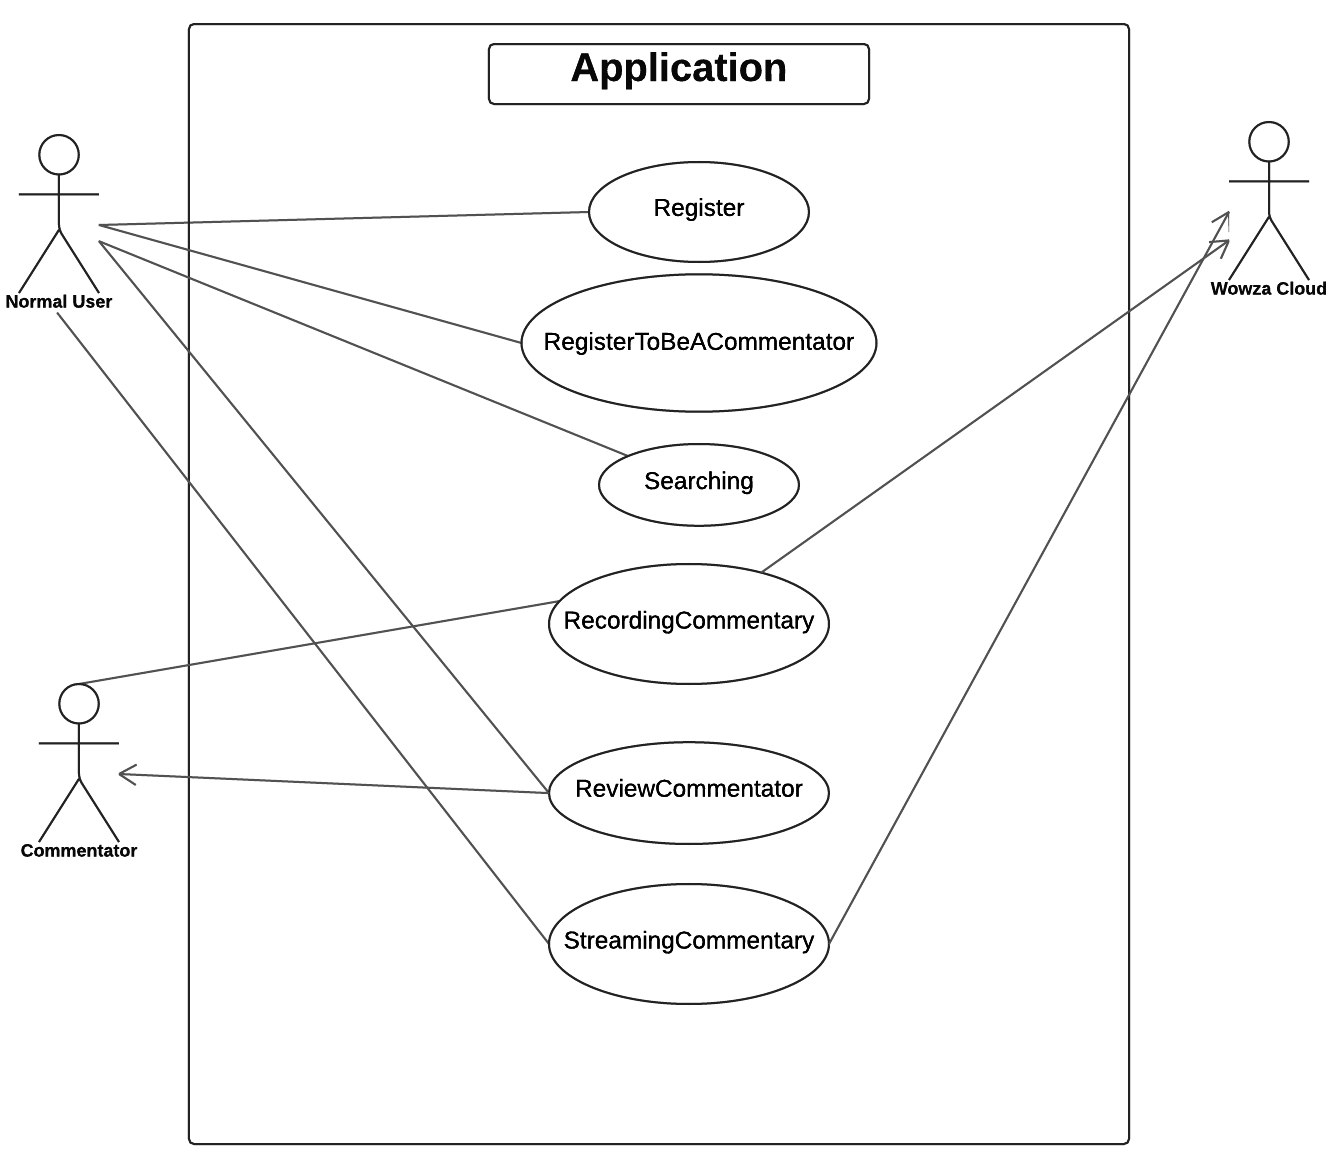
\includegraphics[width=14cm]{use-case-diagram}
    \caption{Application Use Case Diagram}
    \label{fig:use-case-diagram}
\end{figure}
{\large 3.2.2 Use Case Titles}\\
This is the list of use case titles for the application:\\
\noindent Register\hfill RegisterToBeACommentator\\
\noindent Searching\hfill RecordingCommentary\\
\noindent ReviewCommentator\hfill StreamingCommentary\\
{\Large 3.3 Entity-Relationship (ER) Diagram}\\
ER diagrams are graphical representations of entities and their relationship within a system. An entity is an object or concept about which data is stored. A relationship describes how data is shared between two entities.  There are three types of relationships which differs in number of participants involved: one to one, one to many and many to one\textsuperscript{10}. The diagram below will show all the entities involved in the application.\\
\begin{figure}[h]
	\centering
	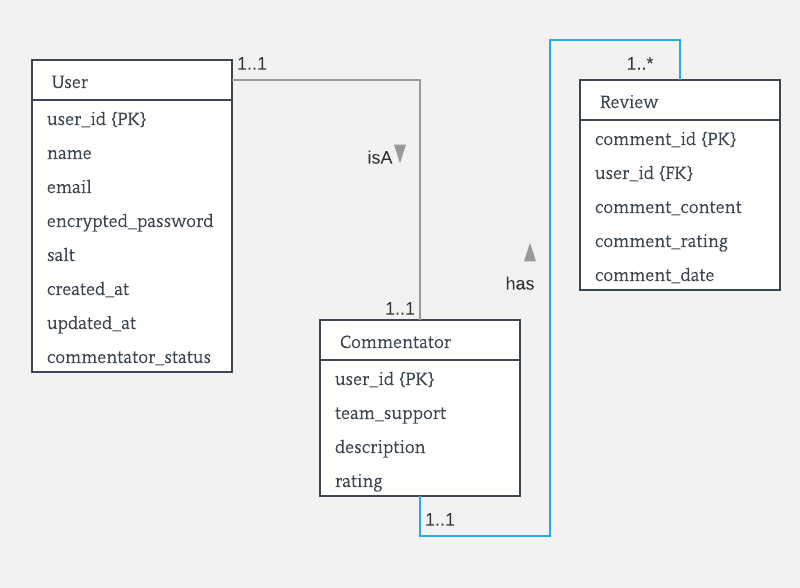
\includegraphics[width=14cm]{er-diagram}
	\caption{Application ER Diagram}
	\label{fig:er-diagram}
\end{figure}
{\huge 4. Design and Implementation}\\
{\Large 4.1 System Architecture}\\
So just any other streaming applications, the system is divided into two main components, the back-end webserver and the Android application itself. The back-end webserver handles user-related functionalities that requires interactions with users' data. The Android application component is the front-end that provides graphical user interface (GUI) and links all the functionalities together to provide users a smooth experience.\\
\autoref{fig:system-architecture} showcases the overall system. The \textbf{Server Side} is shown on the top of the diagram, it consists of only script files to interact with the database that contains all of users' information. The \textbf{Android Application} component is displayed on the bottom of the diagram that, it shows all of the main activities that are involved with the functionalities displayed in the diagram. The bottom row of each cell demonstrates dependencies and arrows represent the flow of execution of the application.\\
\begin{figure}[!h]
	\centering
	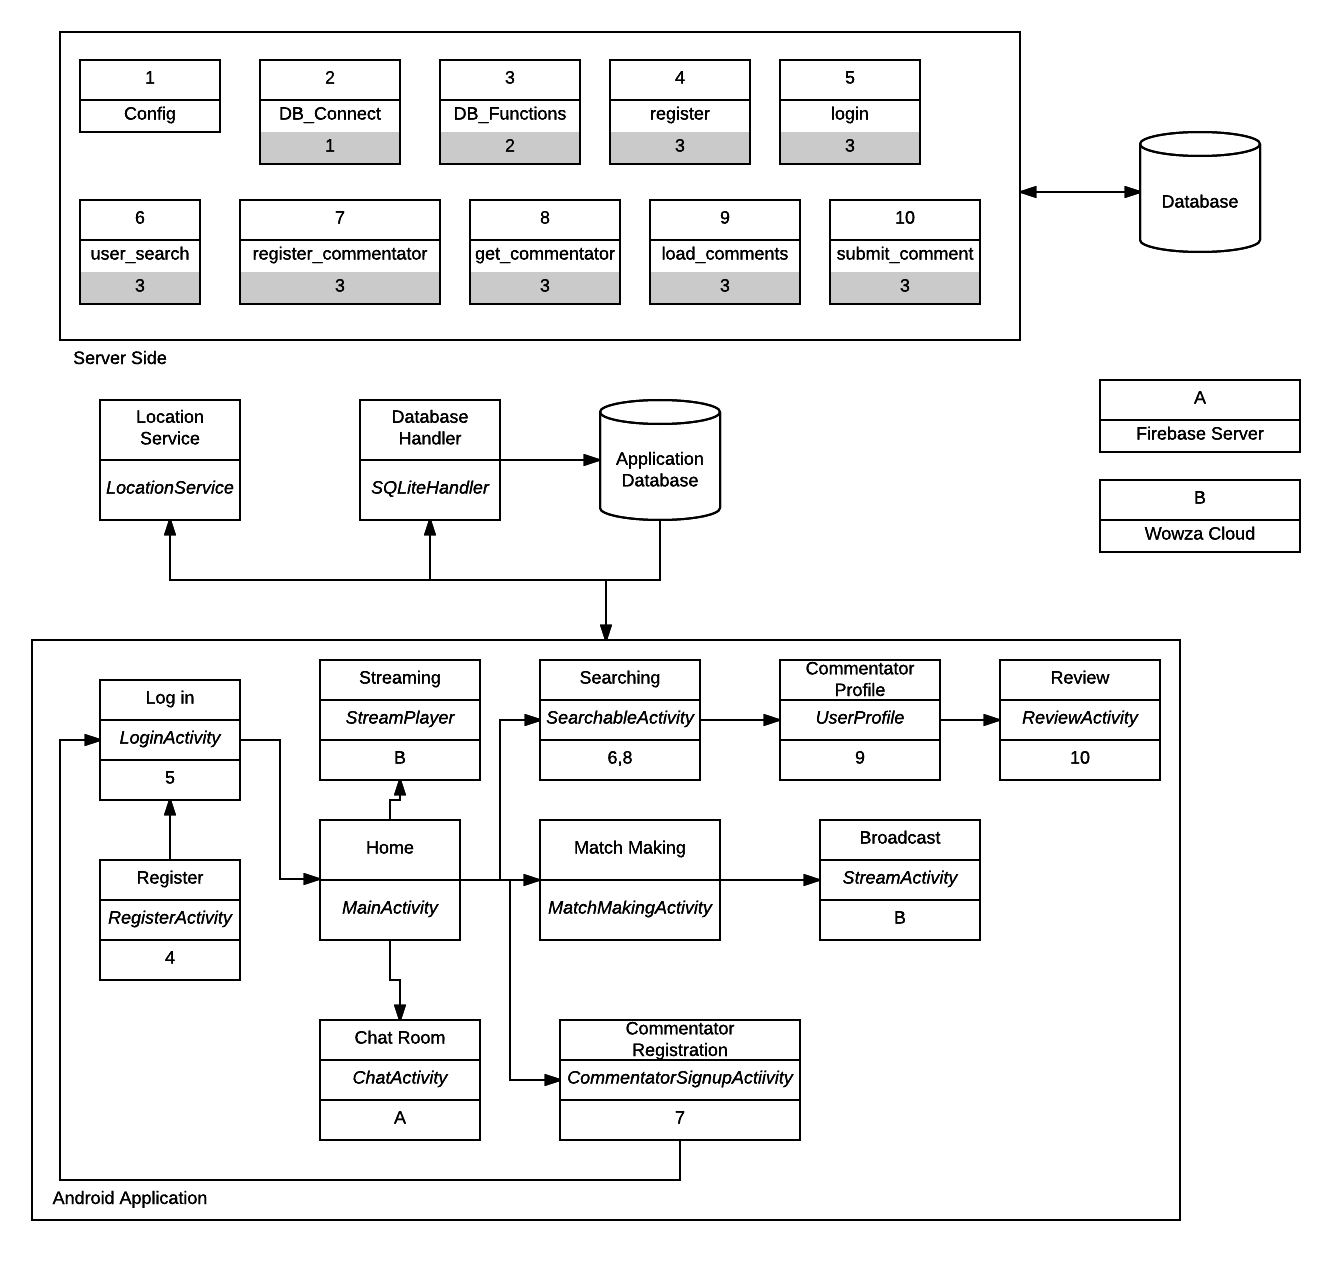
\includegraphics[width=13.5cm]{system-architecture}
	\caption{System Architecture}
	\label{fig:system-architecture}
\end{figure}
{\Large 4.2 Data Flow Diagram}\\
As the application aims to provide users streaming services, understanding of data flow and different components within the streaming cloud are also quite crucial when designing the system.\\
\begin{figure}[!h]
	\centering
	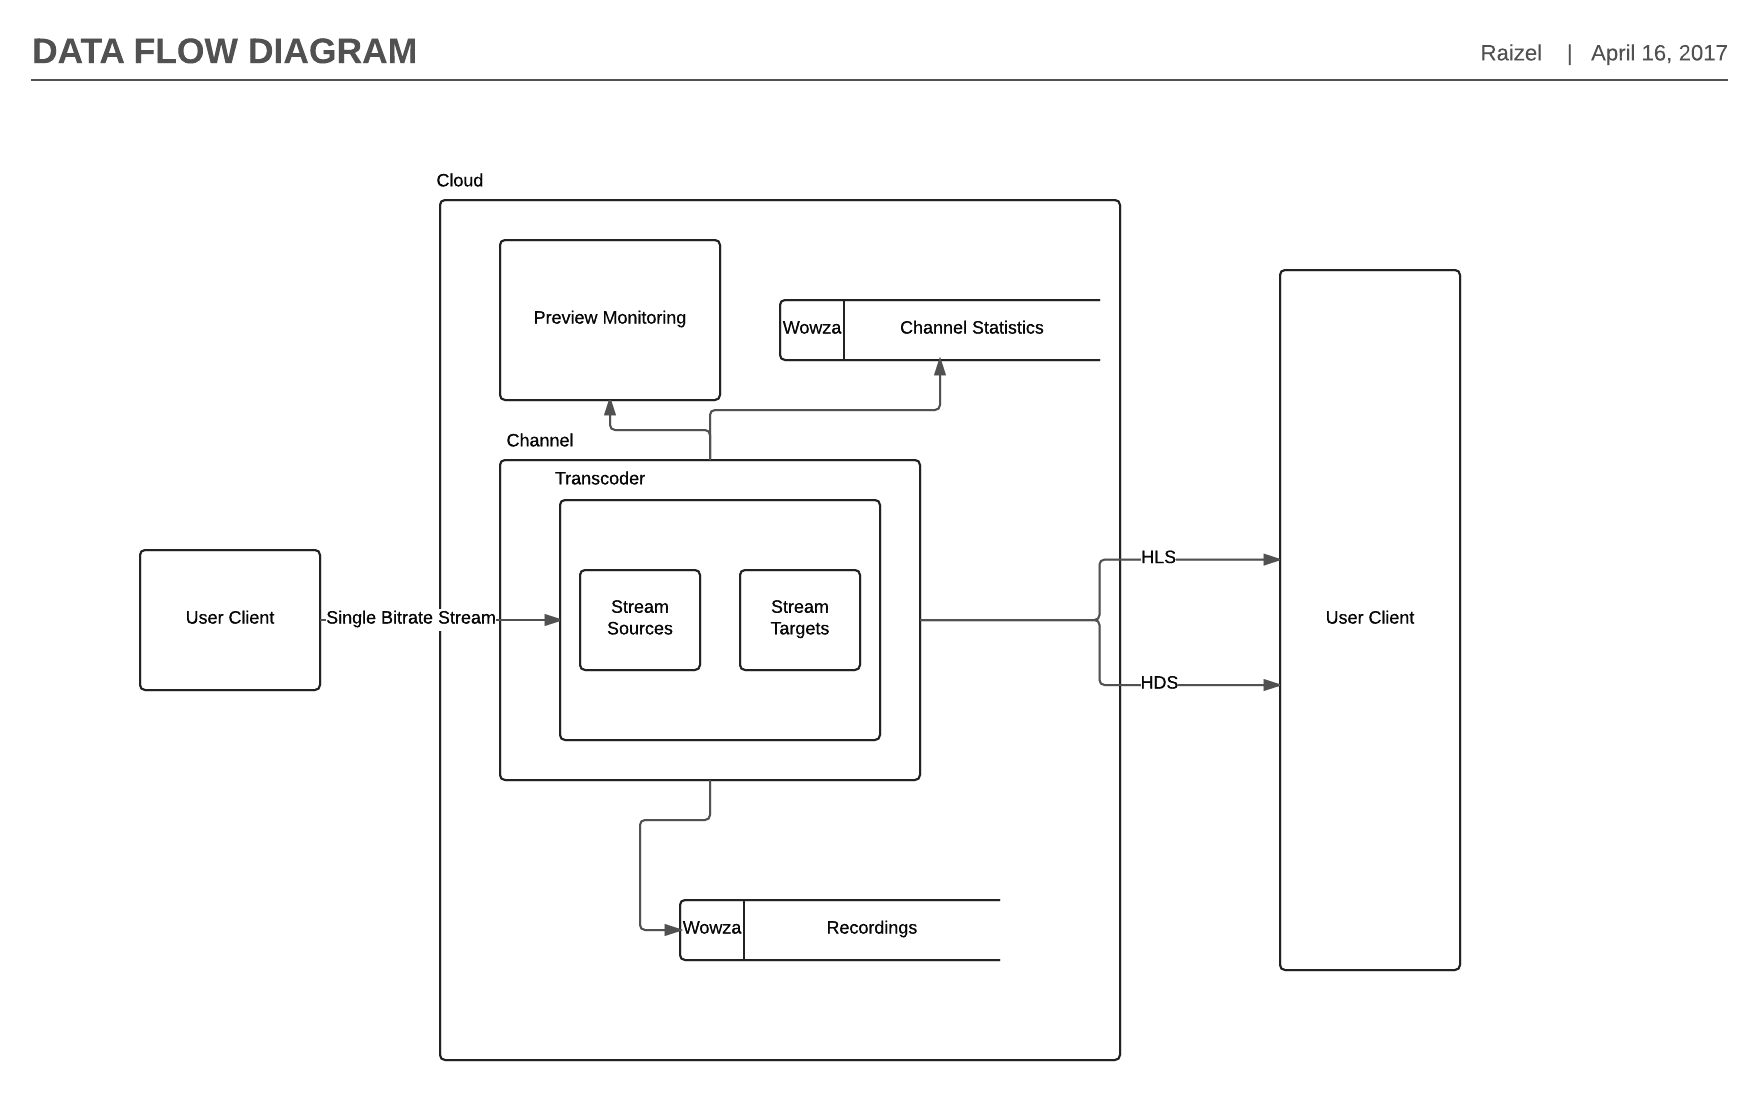
\includegraphics[width=14cm]{data-flow-diagram}
	\caption{Data Flow Diagram}
	\label{fig:data-flow-diagram}
\end{figure}
So the application will send only a single bitrate stream to the channel which can take multiple stream sources at once but can cause congestion. The transcoder is a part of the channel which generates adaptive bitrate passthrough streams and send to specific targets including Facebook Live. This is extended functionality to allow more scalable broadcasts to certain regions or audiences without having geo-blocked channels. Wowza offers two different playback options, Adobe HDS only works with flashplayer which is not supported by Android. Apple HLS is the ideal choice for the system because it is widely supported by a range of different media players available on Android.\\
{\Large 4.3 Application Components}\\
This section will be describing the design of smaller components that make up the Android application.\\
{\large 4.3.1 Broadcasting to Streaming Server}\\
The application relies entirely on Wowza GoCoder SDK to handle the connection to Wowza Streaming Cloud by implementing the \textit{WZStatusCallBack} interface. The workflow is quite simple, it follows a set of procedures to initialise required objects, Below is an overview of the set of functions:
\begin{itemize}
	\item \textbf{initialise()}: This method is self-explanatory, it initialises all required objects. Firstly, it creates a \textit{WowzaGoCoder} (the top level GoCoder API interface) object by giving it a valid Wowza GoCoder SDK key. After that, create an \textit{WZBroadcast} (The broadcaster instance) object along with an \textit{WZBroadcastConfig} (where all credentials to connect to Wowza Streaming Cloud is set, these information are available on user's Wowza Streaming channel) object. Finally an \textit{WZAudioDevice} object that creates an \textit{AudioRecord} instance to record media, which is set to 44.1 kHz sampling rate by default and set to the highest sample rate if the default is not supported, more on this will be available on subsequent section.\\
	\item \textbf{onWZError()}: This method reports any error caused the GoCoder SDK like invalid SDK key.\\
	\item \textbf{onWZStatus()}: This method reports back the status of connection between the device and Wowza Streaming Cloud.\\
\end{itemize} 
\textbf {4.3.1.1 Audio Sampling Rate}\\
Sample rate is the number of samples of audio carried per second measured in Hz or kHz, generally the higher the sample rate the better the quality of audio produced.\textsuperscript{11}. Android's support for audio sample rates varies greatly from device to device and there's also the compromise between size and quality:\\
\begin{itemize}
	\item 48,000 Hz: Used for DVDs and normally is the maximum sample rate supported by Android devices.\\
	\item 44,100 Hz: The sampling rate of audio CDs which reproduce the maximum frequencies of 20,000 Hz, average humans can't really distinguish frequency above 16,000 Hz and only very small portions can hear above 20,000 Hz. Furthermore, this sample rate is supposed to be the only rate that is guaranteed to work across all devices according to Android documents\textsuperscript{12}. However, even though the sample rate is widely supported, it is not guaranteed to work on every single device i.e. Samsung Note 4 doesn't seem to support it. Another reason for using this sample rate as the default is its size, 10 minutes of streaming at 44100 Hz totalled at around 700 KB or only 7 MB for a full football match, while the output is often 10 times this amount so probably there was some sort of encryption involved in the process.\\
	\item 22,050 Hz: reasonably popular for low bit rate MP3s,  often used in: AM radio or situations where perceived quality is unimportant but clarity must be maintained.
	\item 11,025 Hz: Very poor sound quality and can be found in WAV files.
	\item 8,000 Hz: Telephone transmission as it is a good trade-off between quality and bandwidth due to limited bandwidth.
\end{itemize}
{\large 4.3.2 Database}\\
{\textbf {4.3.2.1 Structure}}\\
Due to the nature of the application, data is expired quite quickly, so having a confisticated in-app database is unfit in this situation. However, immutable data used to identify the user should still be stored to avoid unnecessary requests to the server.\\
\textit{user}\\
\begin{tabular}{| c | c | c | c | c |}
\hline
uid (PK) & name & email & commentator & created\_at\\
\hline
\end{tabular}\\
These data is used by the application to identify the user, "commentator" column is used to identify the user's commentator status to check if user has rights to broadcast.\\
{\textbf {4.3.2.2 Implementation}}\\
SQLite Database is a library supported by Android, that implements a server-less, zero-configuration SQL engine database. More specifically, SQLite reads and writes directly to disk files hence requires no server and doesn't require installation, while being quite compact at the same time, library can take up as little space as 500 KB with all features enabled. Furthermore, SQLite is cross-platform and so can be copied directly to different platforms\textsuperscript{13}.\\
The application interacts with the database via a helper class named \textit{SQLiteHandler} that extends \textit{SQLiteOpenHelper} an abstract class that manages database creation and version control. This class contains:
\begin{itemize}
	\item \textbf{onCreate()}: The method is called when database is created the first time, \textit{user} table is created in this method.\\
	\item \textbf{onUpdate()}: typically used for version control, when there's a change to the structure of the table, old \textit{user} table is dropped and it calls \textbf{onCreate()} method to create the new table.\\
	\item \textbf{addUser()}: Quite self-explanatory, this method is used to store user details in the database, the method is called every time the user logs in.\\
	\item \textbf{getUserDetails()}: Fetch user details from the database into a hashmap object and return it.
	\item \textbf{deleteUsers()}: this method calls \textbf{getWritableDatabase()} and delete all entries in the table. This method will be called every time user logs out, so at any instance of time, at max only one user is stored in the database, this helps to simplify system while preventing user details from getting stolen.\\
\end{itemize}
{\large 4.3.3 Location Service}\\
The application uses users' locations to determine whether the user is actually winthin the radius of the stadium when preparing to broadcast. More specifically, users should be within 200 meters (Emirates Stadium is around 17 acres, so this is a reasonable threshold) of the stadium. This is put into place as a measure to prevent users from broadcasting irrelevant contents. Since this is the only purpose of getting users' locations, the application will only check this once because listening to location changes is an intensive process and will waste a lot of battery taking in mind, users will also be broadcasting at the same time. The \textit{LocationService} gets users' whereabouts by implementing \textit{LocationListener} interface that is used for receiving notifications from \textit{LocationManager} when location has changed.\\
On Android, there are two location providers: GPS and Network, each has its own good and bad points.\\
\begin{itemize}
	\item GPS: more accurate but only works outdoors and doesn't respond very fast while consuming more battery.
	\item Network: Determines locations using cellular and wifi signals so it's not as accurate GPS but responds faster, works both indoors and outdoors and also doesn't consume as much battery.
\end{itemize}
The application makes use of both providers, since both speed and accuracy are wanted but not essential. The \textit{getLastBestLocation()} get both locations and compare their times, the newer one is returned.\\
{\large 4.3.4 Connecting to Server Side}\\
The application uses Retrofit to manage transactions between device and the server side which is used thoughout the application, typically functionalities that required interactions with the server side database. Each Retrofit instace is created by caling the \textit{ServiceGenerator} class, the \textit{Datanase} interface is created to contain all the model POST requests (parameters they take, lniks to scripts they call etc.). Retrofit allows both asynchronous and synchronous requests, but since synchronous calls are executed on the main thread therefore UI blocks during request execution reduces application's reponsiveness so in the application all requests are asynchronous. Whether asynchronous and synchronous, they both follow a certain procedure, for our application, a \textit{Database} instance is created by calling \textit{ServiceGenerator} to create a Retrofit instance and call \textit{create(Database.class)} on that instance. After that, the application simply calls the required method from the interface and call \textit{enqueue} to make a request on background thread. In order to get the response, the application simple calls \textit{response.body()} on \textit{onResponse()} method if the request is successful or handle the error on \textit{onFailure()} in case the request was unsuccessful.\\
{\Large 4.4 Application Components}\\
{\large 4.4.1 Server Database}\\
{\textbf 4.4.1.1 Structure}\\
Database normalisation has been performed to reduce data redundancy and improve data integrity to minimise potential errors occurs when inserting, updating or deleting data.\\
\begin{itemize}
	\item \textbf{1st Normal Form}: Database contains only atomic values and there are no repeating groups\textsuperscript{14}.
	\item \textbf{2nd Normal Form}: To satisfy this, database must be in first normal form and all non-key attributes are dependent on the primary key.
	\item \textbf{3rd Normal Form}: Database is in second normal form and there are no transistive functional dependency i.e. an attribute is dependent on another non-primary key attribute which in turns is dependent on the primary key.
\end{itemize}
\textit{users}
\begin{tabular}{| c | c | c | c | c | c | c |}
\hline
user\_id (PK) & name & email & commentator\_status & encrypted\_password & salt & created\_at\\
\hline
\end{tabular}
\textit{commentators}\\
\begin{tabular}{| c | c | c | c |}
\hline
user\_id (PK) & team\_support & description & rating\\
\hline
\end{tabular}\\
\textit{comments}
\begin{tabular}{| c | c | c | c | c |}
\hline
comment\_id (PK) & user\_id (FK) & comment\_content & comment\_rating & comment\_date\\
\hline
\end{tabular}
{\textbf 4.4.1.2 Implementation}\\
All interactions with the database use prepared statements\textsuperscript{15} which are very useful against SQL injections. The prepared works as follows:
\begin{itemize}
	\item \textit{prepare()}: Create an SQL statement template without specified values which is sent to the database for syntax checks and initialises resources for later use.
	\item \textit{execute()}: The client binds parameter values using \textit{bind_param()} and calls \textit{execute()} to send it to the database (since values are sent seperately from query, it cannot interfere with it hence useful against SQL injections) which will create a statement from the template with bound values and execute it.
\end{itemize}
There are multiple benefits for using prepared statements besides the fact that they are useful against SQL injections. Firstly, these statements can be executed repeatedly with different values by changing the bound variable. Another benefit is that it cuts out parsing and validation which makes it runs faster.\\
{\huge References}\\[0.5cm]
\textsuperscript{1}"Android Developers". Developer.android.com. N.p., 2007. Web. 15 Mar. 2017.\\
\textsuperscript{2}Tamada, Ravi and Ravi Tamada. "Android Login And Registration With PHP, Mysql And Sqlite". androidhive. N.p., 2016. Web. 16 Mar. 2017.\\
\textsuperscript{3}"Retrofit — Getting Started And Creating An Android Client". Futurestud.io. N.p., 2015. Web. 16 Mar. 2017.\\
\textsuperscript{4}"How To Create An Android Chat App Using Firebase". code.tutsplus. N.p., 2016. Web. 16 Mar. 2017.\\
\textsuperscript{5}Tamada, Ravi et al. "Android Sliding Menu Using Navigation Drawer". androidhive. N.p., 2013. Web. 16 Mar. 2017.\\
\textsuperscript{6}"Stack Overflow". Stackoverflow.com. N.p., 2008. Web. 16 Mar. 2017.\\
\textsuperscript{7}Mobdro. Mobdro, 2016. Print.\\
\textsuperscript{8}Ustream. Ustream an IBM Company, 2016. Print.\\
\textsuperscript{9}UK TVNow. UKTVNow; 2015. \\
\textsuperscript{10}Beal V. What is Entity Relationship Diagram? Webopedia Definition [Internet]. Webopedia. 2017 [cited 14 April 2017]. Available from: \url {http://www.webopedia.com/TERM/E/entity_relationship_diagram.html}\\
\textsuperscript{11}Sample Rates - Audacity Wiki [Internet]. Wiki.audacityteam.org. 2016 [cited 16 April 2017]. Available from: \url{http://wiki.audacityteam.org/wiki/Sample_Rates}\\
\textsuperscript{12}AudioRecord | Android Developers [Internet]. Developer.android.com. 2017 [cited 16 April 2017]. Available from: \url{https://developer.android.com/reference/android/media/AudioRecord.html}\\
\textsuperscript{13}About SQLite [Internet]. Sqlite.org. 2017 [cited 17 April 2017]. Available from: \url{https://www.sqlite.org/about.html}\\
\textsuperscript{14}Database Normalization [Internet]. 1keydata.com. 2015 [cited 18 April 2017]. Available from: \url{http://www.1keydata.com/database-normalization/}\\
\textsuperscript{15}PHP Prepared Statements [Internet]. W3schools.com. 2017 [cited 18 April 2017]. Available from: \url{https://www.w3schools.com/php/php_mysql_prepared_statements.asp}\\
\end{flushleft}
\end{document}
